% If you are LaTeX 2.09 user:
% \documentstyle[twocolumn,ncsp16,ascmac,a4paper]{article}
%
\documentclass[twocolumn,a4paper]{article}
\usepackage[colorlinks, urlcolor=blue,
	pdffitwindow, bookmarksopen,
	filecolor=blue,
	bookmarksopenlevel=0,
	pdfpagelayout=SinglePage, dvipdfm]{hyperref} 
\usepackage{ncsp16} %% !! Strongly recommended to use it
\usepackage{color}
\usepackage{ascmac}
\usepackage{graphicx}
\graphicspath{{./Figure/}}

\begin{document}

\title{All Optical AND Gate Using Photonic Crystal Quantum-Dot Semiconductor Optical Amplifiers}

\name{Takuma Matsumoto, Gou Hosoya, and Hiroyuki Yashima}
%%% The order of name is first name and family name. 
%%% First characters in each of them should be written by a capital letter, for example, Mikio Hasegawa, not Mikio HASEGAWA. 
%%% If many authors are required to listed and more than one row is needed, use the following list.  
% \name{
% \begin{tabular}{c}
% Iker Casillas, Sergio Ramos, Carles Puyol, Maicon, Philipp Lahm, Andres Iniesta, Xavi, \\Bastian Schweinsteiger, Wesley Sneijder, Diego Forlan, David Villa, and Vicente del Bosque
% \end{tabular}
% }

\address{
\begin{tabular}{c}
%%% !! Authors should fill all the lists of the following information. 
Tokyo University of Science\\
6-3-1, Shinjuku Katsushika-ku, Tokyo, 125-8585 Japan\\
Phone/FAX:+81-3-5876-1717\\
E-mail:  4416630@ed.tus.ac.jp
\end{tabular}
}

%%%%
%%%% If more than one affiliations are needed, use the following list. 
%%%%

% \name{Mikio Hasegawa$^1$, Mikio Hasegawa$^2$ and Mikio Hasegawa$^1$}

% \address{
% \begin{tabular}{c}
% $^1$
%Tokyo University of Science\\
%6--3--1, niijyuku, Katsushika-ku, Tokyo, 125--8585 Japan\\
%Phone/FAX:+81-999-99-9999\\
%E-mail: tpc16@ncsp.jp
% \end{tabular}
% \begin{tabular}{c}
% $^2$
%Tokyo University of Science\\
%6--3--1, niijyuku, Katsushika-ku, Tokyo, 125--8585 Japan\\
%Phone/FAX:+81-999-99-9999\\
%E-mail: tpc16@ncsp.jp
% \end{tabular}
% }

\maketitle

\section*{Abstract}

We propose all optical AND gate using photonic crystal quantum-dot semiconductor optical amplifiers(PC-QDSOA). We evaluate the input-output characteristics by numerical analysis. It is shown that the proposed AND gate is well operated at 160Gbps. Also, 

\section{Introduction}
The demand of telecommunications is grown with the spread of mobile phone users. To cope with the demand, ultrafast light wave communications and networks are essential. In current optical communication network, signal processing technology is used for electrical signal only, and thus, processing electric signal limits the efficiency of current optical communication network{\cite{App}}. So, all optical signal processing  without electrical processing has been developed and the development of all optical devices are required. In recent researches, 

In this paper we propose an all optical error correcting encoder and decoder using horizontal and vertical parity checks. We numerically analyze the encoder and decoder to check input and output waveform of each systems. In addition, we show the performance and efficiency of the proposed code.

\section{Optical Device}
\subsection{PC-QDSOA}


\subsection{All Optical AND Gate}
Fig.{\ref{figure:xor_gate}} shows the configuration of all optical XOR gate using quantum dot semiconductor optical amplifier(QD-SOA){\cite{Omar}}--{\cite{Ultrafast}}. Two QD-SOA devices and 3dB couplers compose all optical XOR gate. QD-SOA is an optical device used for optical amplifier and modulates phase of output optical signal depending on input optical signal strength.

First, the $1 \times 2$ coupler separates clock signal into two waveguides. The clock signal traveling through the upper waveguide and the lower waveguide are fed into the QD-SOA1 and QD-SOA2, respectively. The QD-SOA1 and QD-SOA2 modulate the phase of clock signal by $\phi_{A}$ and $\phi_{B}$ according to input optical signal A and B, respectively. If the phase of the output signal of QD-SOA1 is equal to that of QD-SOA2, the output signals are coupled by the $2 \times 1$ coupler and cancel each other, and thus, the output of the coupler is ``0''. If the phase of the output signal of the QD-SOA1 is different from that of the QD-SOA2 by $\pi$, the output signals are coupled by $2 \times 1$ coupler and the output signal is obtained as ``1''. Thus, table {\ref{table:xor_table}} shows a truth table of all optical XOR gate.

\begin{figure}[htbp]
\begin{center}
  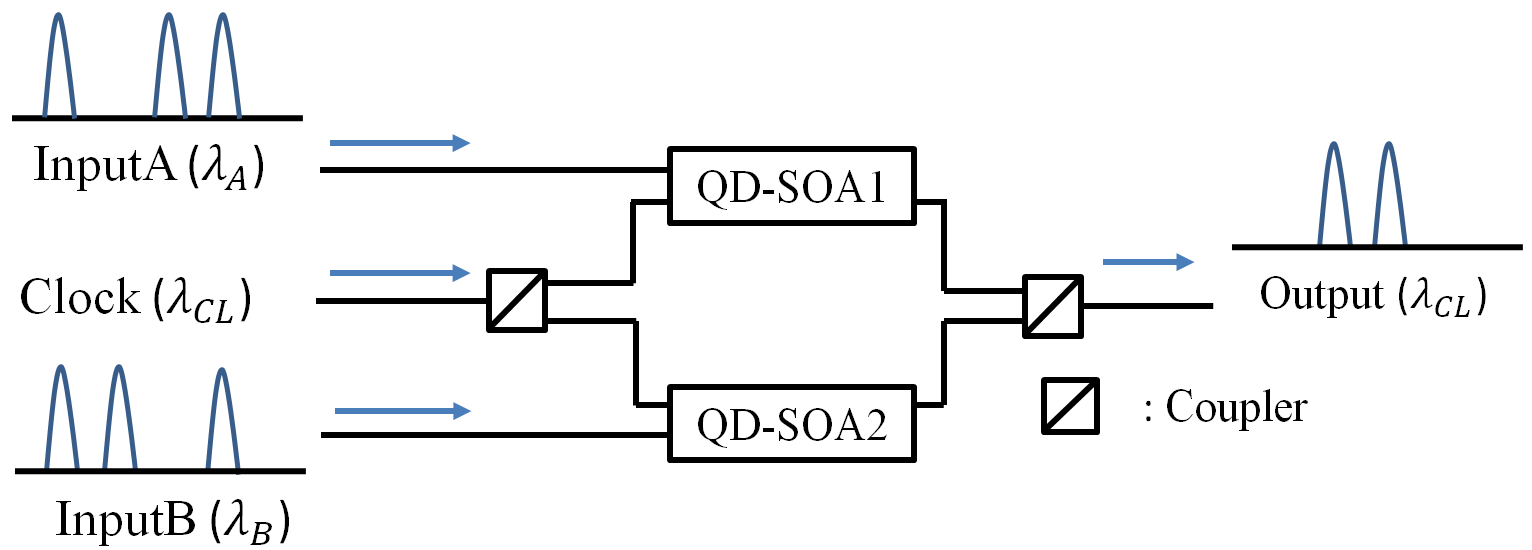
\includegraphics[width=80mm]{QDSOA_Based_XOR.eps}
  \caption{The configuration of QD-SOA based XOR gate}
 \label{figure:xor_gate}
\end{center}
\end{figure}

\renewcommand{\arraystretch}{1.5}
\begin{table}[htbp]
\begin{center}
 \small
 \caption{A truth table of all optical XOR gate}
 \label{table:xor_table}
 \begin{tabular}{c c c}
  \hline
  InputA & InputB & Output \\
  \hline
  $0$ & $0$ & $0$ \\
  $0$ & $1$ & $1$ \\
  $1$ & $0$ & $1$ \\
  $1$ & $1$ & $0$ \\
  \hline
  \end{tabular}
\end{center}
\end{table}
\renewcommand{\arraystretch}{1.0}

\newpage

\subsection{All Optical AND Gate}
Fig.{\ref{figure:and_gate}} shows the configuration of all optical AND gate{\cite{80Gbps}}. Although, the configuration is similar to that of all optical XOR gate, the positions of input signal B and clock signal are replaced. If the input signal B is ``0'', the coupler does not output signal. If the input signal B is ``1'' and input signal A is ``0'', the phase of signal traveling through upper waveguide is different from that of lower waveguide by $\pi$, hence the coupler outputs ``0''. If the input signal A and B are ``1'', the phase of the upper waveguide is different from that of the lower waveguide by $\pi$, hence the coupler outputs ``1''. Thus, table {\ref{table:and_table}} shows a truth table of all optical AND gate.

\begin{figure}[htbp]
\begin{center}
  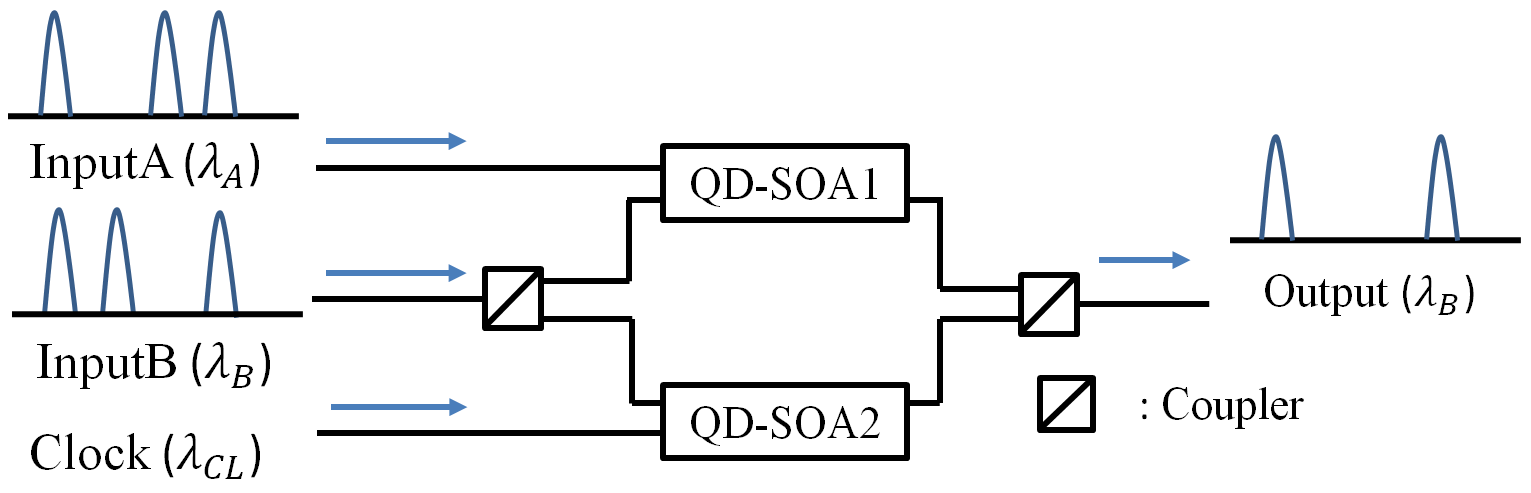
\includegraphics[width=80mm]{QDSOA_Based_AND.eps}
  \caption{The configuration of QD-SOA based AND gate}
 \label{figure:and_gate}
\end{center}
\end{figure}

\renewcommand{\arraystretch}{1.5}
\begin{table}[htbp]
\begin{center}
 \small
 \caption{A truth table of all optical AND gate}
 \label{table:and_table}
 \begin{tabular}{c c c}
  \hline
  InputA & InputB & Output \\
  \hline
  $0$ & $0$ & $0$ \\
  $0$ & $1$ & $0$ \\
  $1$ & $0$ & $0$ \\
  $1$ & $1$ & $1$ \\
  \hline
  \end{tabular}
\end{center}
\end{table}
\renewcommand{\arraystretch}{1.0}

\section{All Optical Error Correcting Code Using Horizontal and Vertical Parity Checks}
\subsection{Horizontal and Vertical Parity Checks}
Fig.{\ref{figure:checks}} shows the placement of horizontal and vertical parity checks. We use 8-bit-length checks composed of 4-bit-length data and 4-bit-length parity. $x_1,x_2,x_3,x_4$ are referred to as data bit and $x_5,x_6,x_7,x_8$ are referred to as parity bit. Parity bits are calculated as the following equation.
\begin{eqnarray}
  x_5 = x_1 \oplus x_2 \\
  x_6 = x_3 \oplus x_4 \\
  x_7 = x_1 \oplus x_3 \\
  x_8 = x_2 \oplus x_4 
\end{eqnarray}

\begin{figure}[htbp]
\begin{center}
  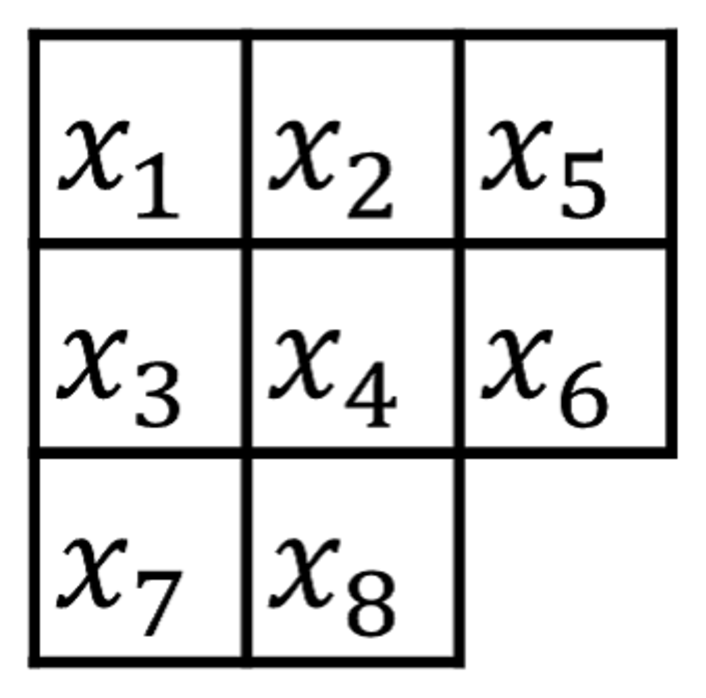
\includegraphics[width=22mm]{Parity.eps}
  \caption{Horizontal and vertical parity checks}
  \label{figure:checks}
\end{center}
\end{figure}

\subsection{Encoder}
Fig.{\ref{figure:encoder}} shows the block diagram of the encoder. First, the $1 \times 5$ splitter separates information signal into five waveguides. The four of five waveguides are used for generating parity. Delay elements are used to adjust the timing of each data bits and they are fed into the $1 \times 2$ splitters. Each XOR gates generate one bit of parity and after delaying each bits, the $4 \times 1$ power combiner combines each bits to convert the parallel signal to serial one. Finally, the $2 \times 1$ power combiner combines transmitted signal and generated parity to generate encoded code.

\begin{figure}[htbp]
\begin{center}
  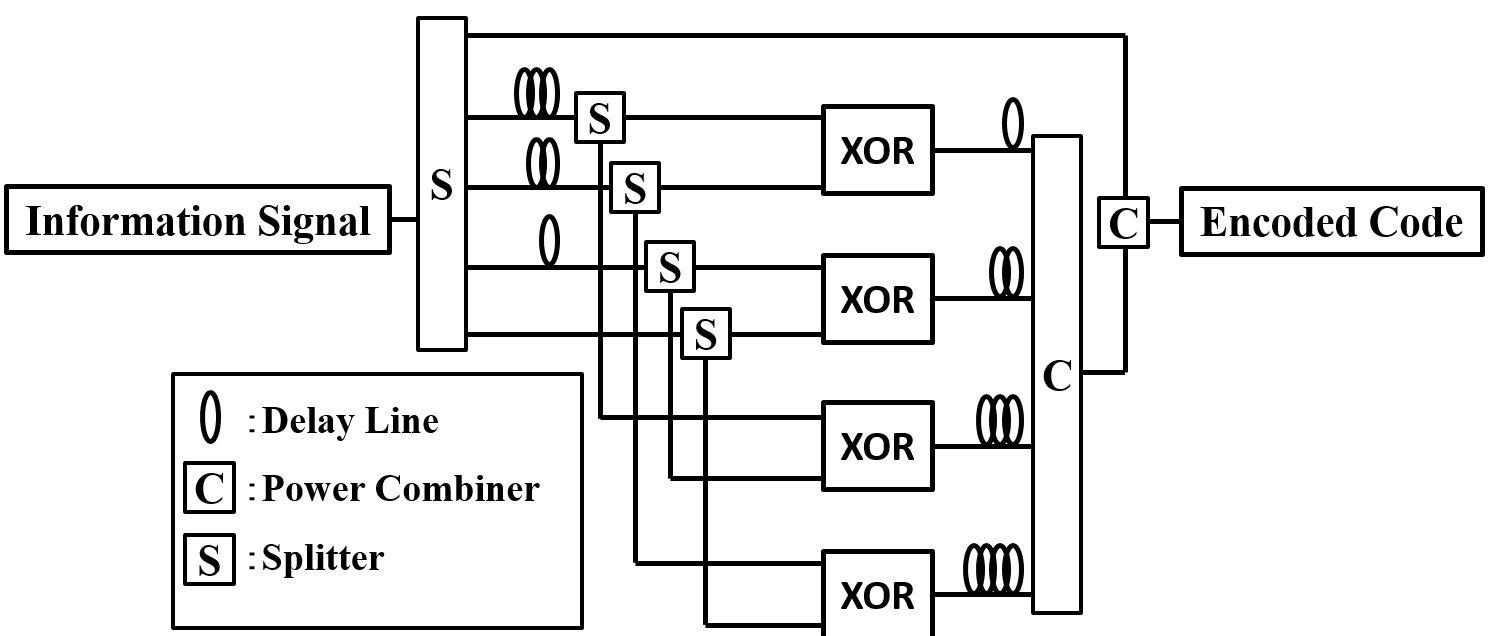
\includegraphics[width=80mm]{Encoder.eps}
  \caption{The block diagram of encoder}
 \label{figure:encoder}
\end{center}
\end{figure}

\subsection{Decoder}
Fig.{\ref{figure:decoder}} shows the block diagram of the decoder. First, the $1 \times 3$ splitter separates received signal into three waveguides. Filter1 picks out only the parity bits in received signal and filter2 picks out only the data bits in received signal. The data bits outputted from filter2 generate parity. The received parity and the generated parity are fed into XOR gate to generate error pattern. We can find out which bit is wrong according to error pattern. If one of the data bits in received signal is wrong, error pattern has two bits whose power is ``1''. The error pattern signal is fed into the $1 \times 4$ splitter and signals travel through four waveguides. After delay elements adjust the timing of each data bits and they are fed into the $1 \times 2$ splitters, AND gates  generate the signal representing which bit is error. The $4 \times 1$ power combiner combines generated signal to convert parallel signal to serial one. Finally, the generated signal and received signal are fed into XOR gate to generate error corrected code.

\begin{figure*}[htbp]
\begin{center}
  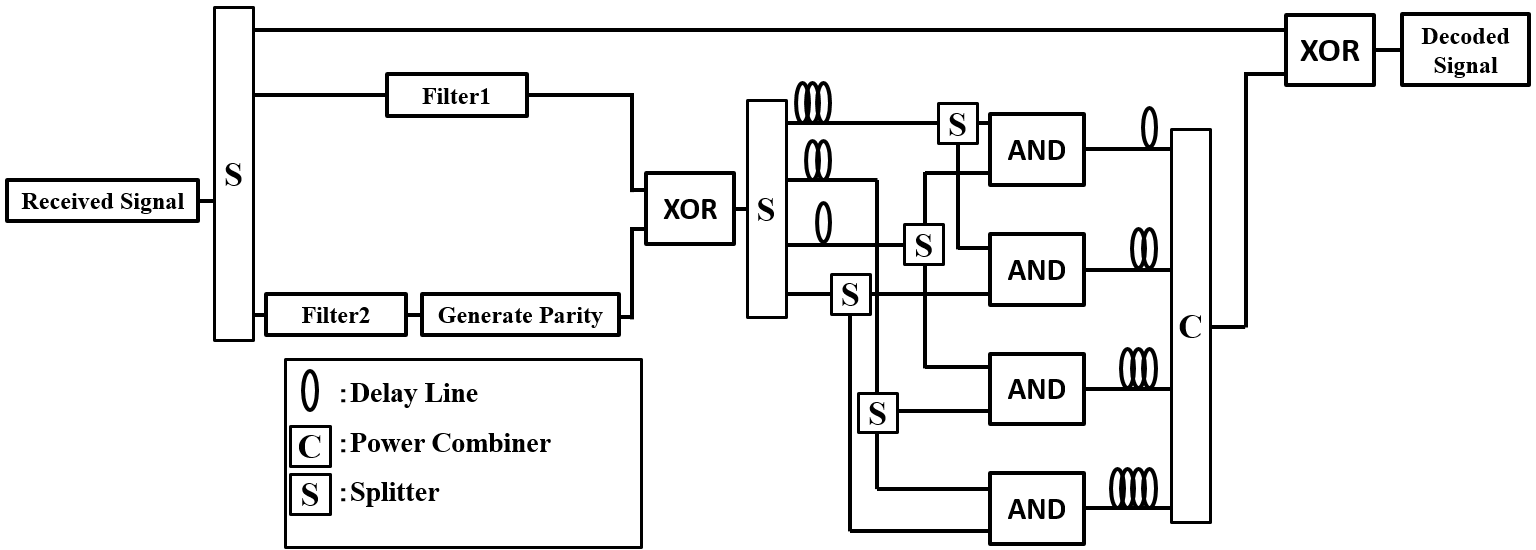
\includegraphics[width=140mm]{Decoder.eps}
  \caption{The block diagram of decoder}
  \label{figure:decoder}
\end{center}
\end{figure*}

\newpage

\section{Results and Discussion}
We use Optisystem13.0.0 and MATLAB R2014a to numerically analyze the behavior of each optical devices at 160Gbps. We use rate equation and transfer matrix method (TMM) to numerically analyze QD-SOA{\cite{Rostami}}. The parameters used for the QD-SOA employed in this paper are shown in table {\ref{table:param}}.

\renewcommand{\arraystretch}{1.5}
\begin{table}[htbp]
\begin{center}
 \small
 \caption{The device parameters}
 \label{table:param}
 \begin{tabular}{c c c}
  \hline
  Description & Value & Unit \\
  \hline
  active medium length & $2.0 \times 10^{-3}$ & $m$ \\
  effective thickness of the active layer & $ 0.25 \times 10^{-6}$ & $m$ \\
  effective width of the active layer & $ 3.0 \times 10^{-6}$ & $m$ \\
  surface density of QDs & $ 5.0 \times 10^{14}$ & $m^{-2}$ \\
  electron relaxation time (WL to ES) & $ 3.0 \times 10^{-12}$ & $s$ \\
  electron escape time (ES to WL) & $ 1.0 \times 10^{-9}$ & $s$ \\
  spontaneous radiative lifetime in WL & $ 2.0 \times 10^{-9}$ & $s$ \\
  electron relaxation time (ES to GS) & $ 0.16 \times 10^{-12}$ & $s$ \\
  electron escape time (GS to ES) & $ 1.2 \times 10^{-12}$ & $s$ \\
  spontaneous radiative lifetime in GS & $ 0.4 \times 10^{-9}$ & $s$ \\
  injection current & $ 3.0 \times 10^{-2}$ & $A$ \\
  maximum modal gain & $ 3.0 \times 10^{2}$ & $m^{-1}$ \\
  line width enhancement factor & $ 2.0 \times 10^{2}$ & $-$ \\
  absorption coefficient & $ 3.0 \times 10^{2}$ & $m^{-1}$ \\
  \hline
\end{tabular}
\end{center}
\end{table}
\renewcommand{\arraystretch}{1.0}

Fig.{\ref{figure:send_compare}} shows the information signal fed into the encoder and the encoded signal at the encoder output. The information signal patterns are ``1110'' and ``0110'' as shown in fig.{\ref{figure:send_compare}(a), and the encoded signal patterns are ``11100101'' and ``01101111'' as shown in fig.{\ref{figure:send_compare}}(b). Fig.{\ref{figure:passive_compare}} shows a received signal and decoded signal. The received signal patterns are ``11110101'' and ``00101111'' as shown in fig.{\ref{figure:passive_compare}}(a). Fig.{\ref{figure:passive_compare}}(a) shows error added received signal corresponding to fig.{\ref{figure:send_compare}}(b). The fourth bit of first pattern is error turned from ``0'' to ``1'' and the second bit of second pattern is error turned from ``1'' to ``0''. The first pattern and second pattern of the decoded signal are ``11100101'' and ``01101111'' respectively, as shown in fig.{\ref{figure:passive_compare}}(b). As a result, the encoder generates code and the decoder corrects error occurred signal at 160Gbps.

\begin{figure}[htbp]
\begin{center}
  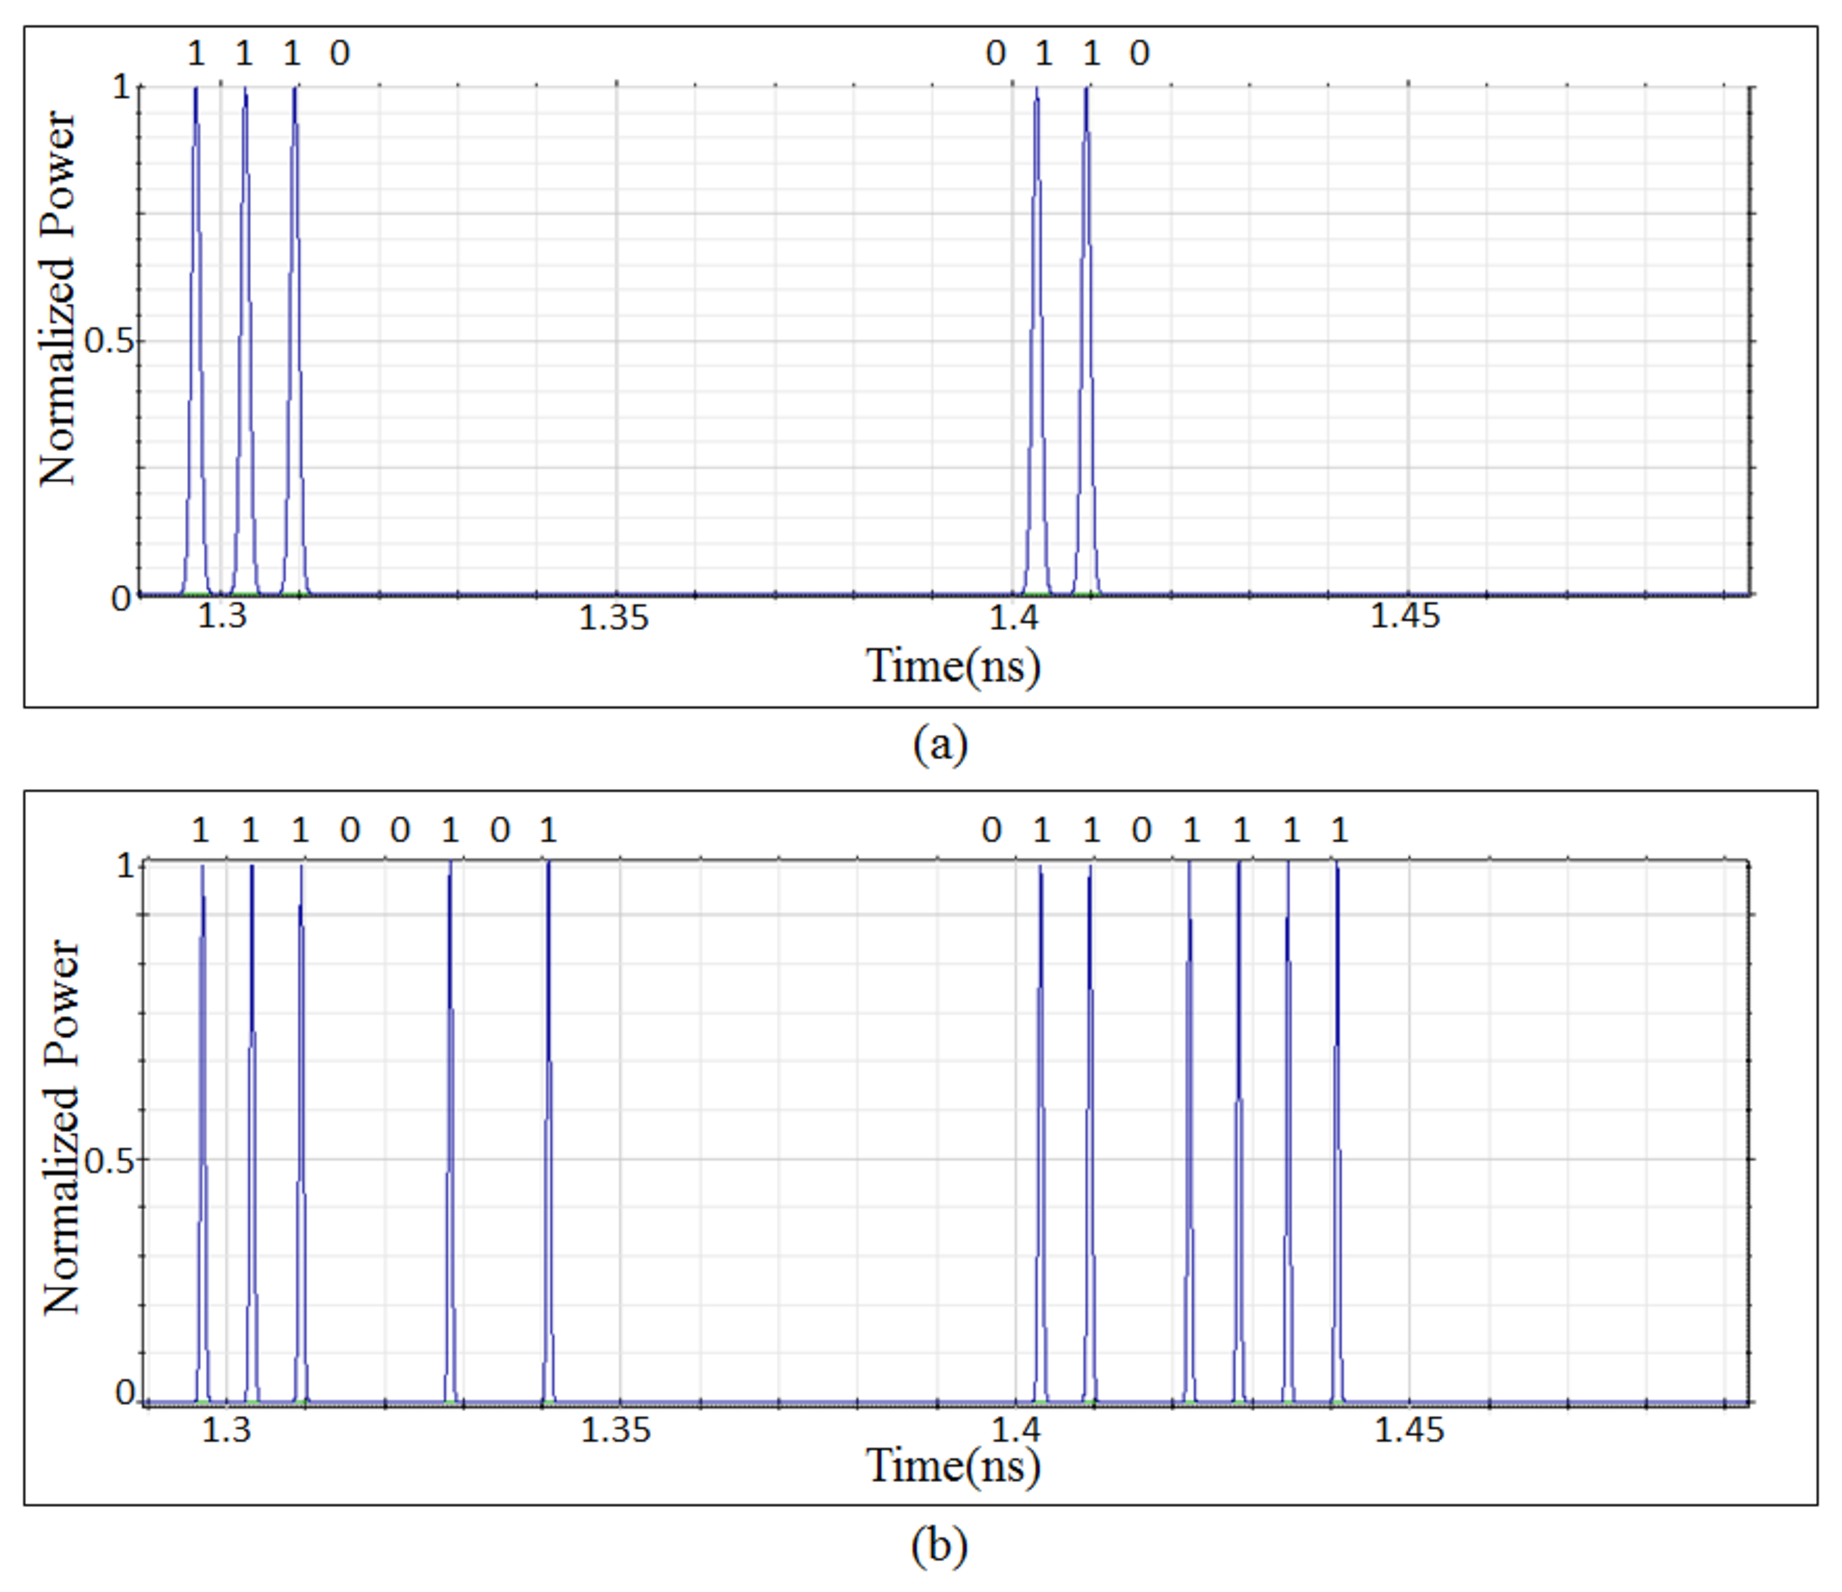
\includegraphics[width=80mm]{send_compare.eps}
  \caption{The waveforms of information signal (a) and encoded code (b) }
  \label{figure:send_compare}
\end{center}
\end{figure}

\begin{figure}[htbp]
\begin{center}
  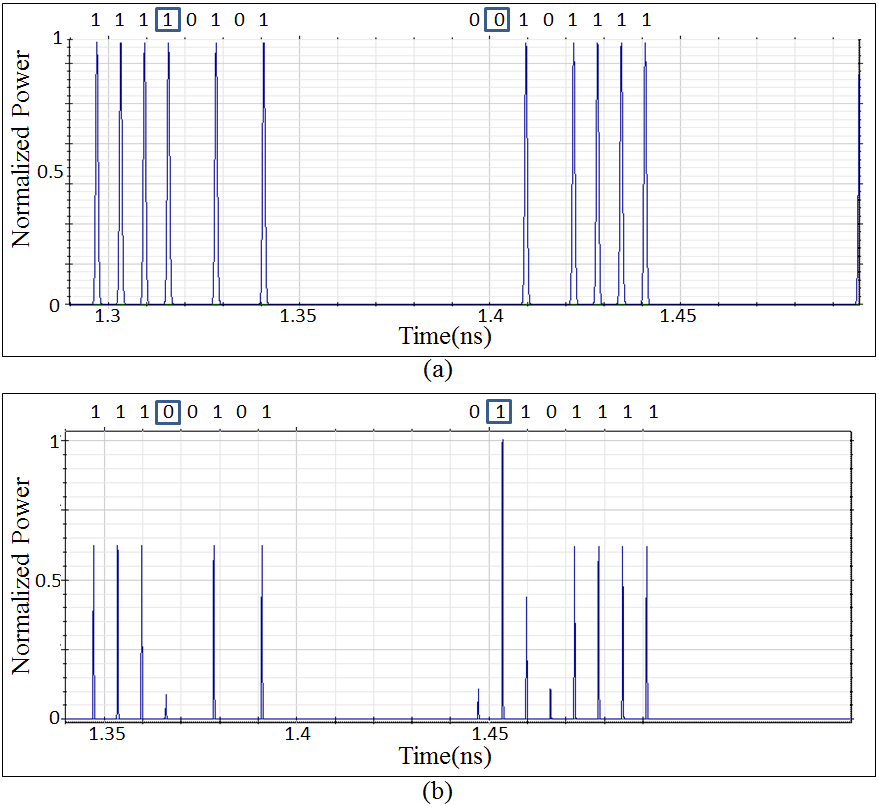
\includegraphics[width=80mm]{passive_compare.eps}
  \caption{The waveforms of received signal (a) and decoded signal (b) }
  \label{figure:passive_compare}
\end{center}
\end{figure}

\newpage

We use eye diagram and obtain extinction ratio as appropriate metrics. The equation of extinction ratio is $ER(dB)=10log_{10}(P^{1}_{\min}/P^{0}_{\max})$ where $P^{1}_{\min}$ is minimum power of signal representing ``1'' and $P^{0}_{\max}$ is maximum power of signal representing ``0''. Fig.{\ref{figure:eyedia}} shows an eye diagram of the decoded signal. We show the proposed system is effective according to 5.72(dB) extinction ratio{\cite{Gayen}}.

\begin{figure}[htbp]
\begin{center}
  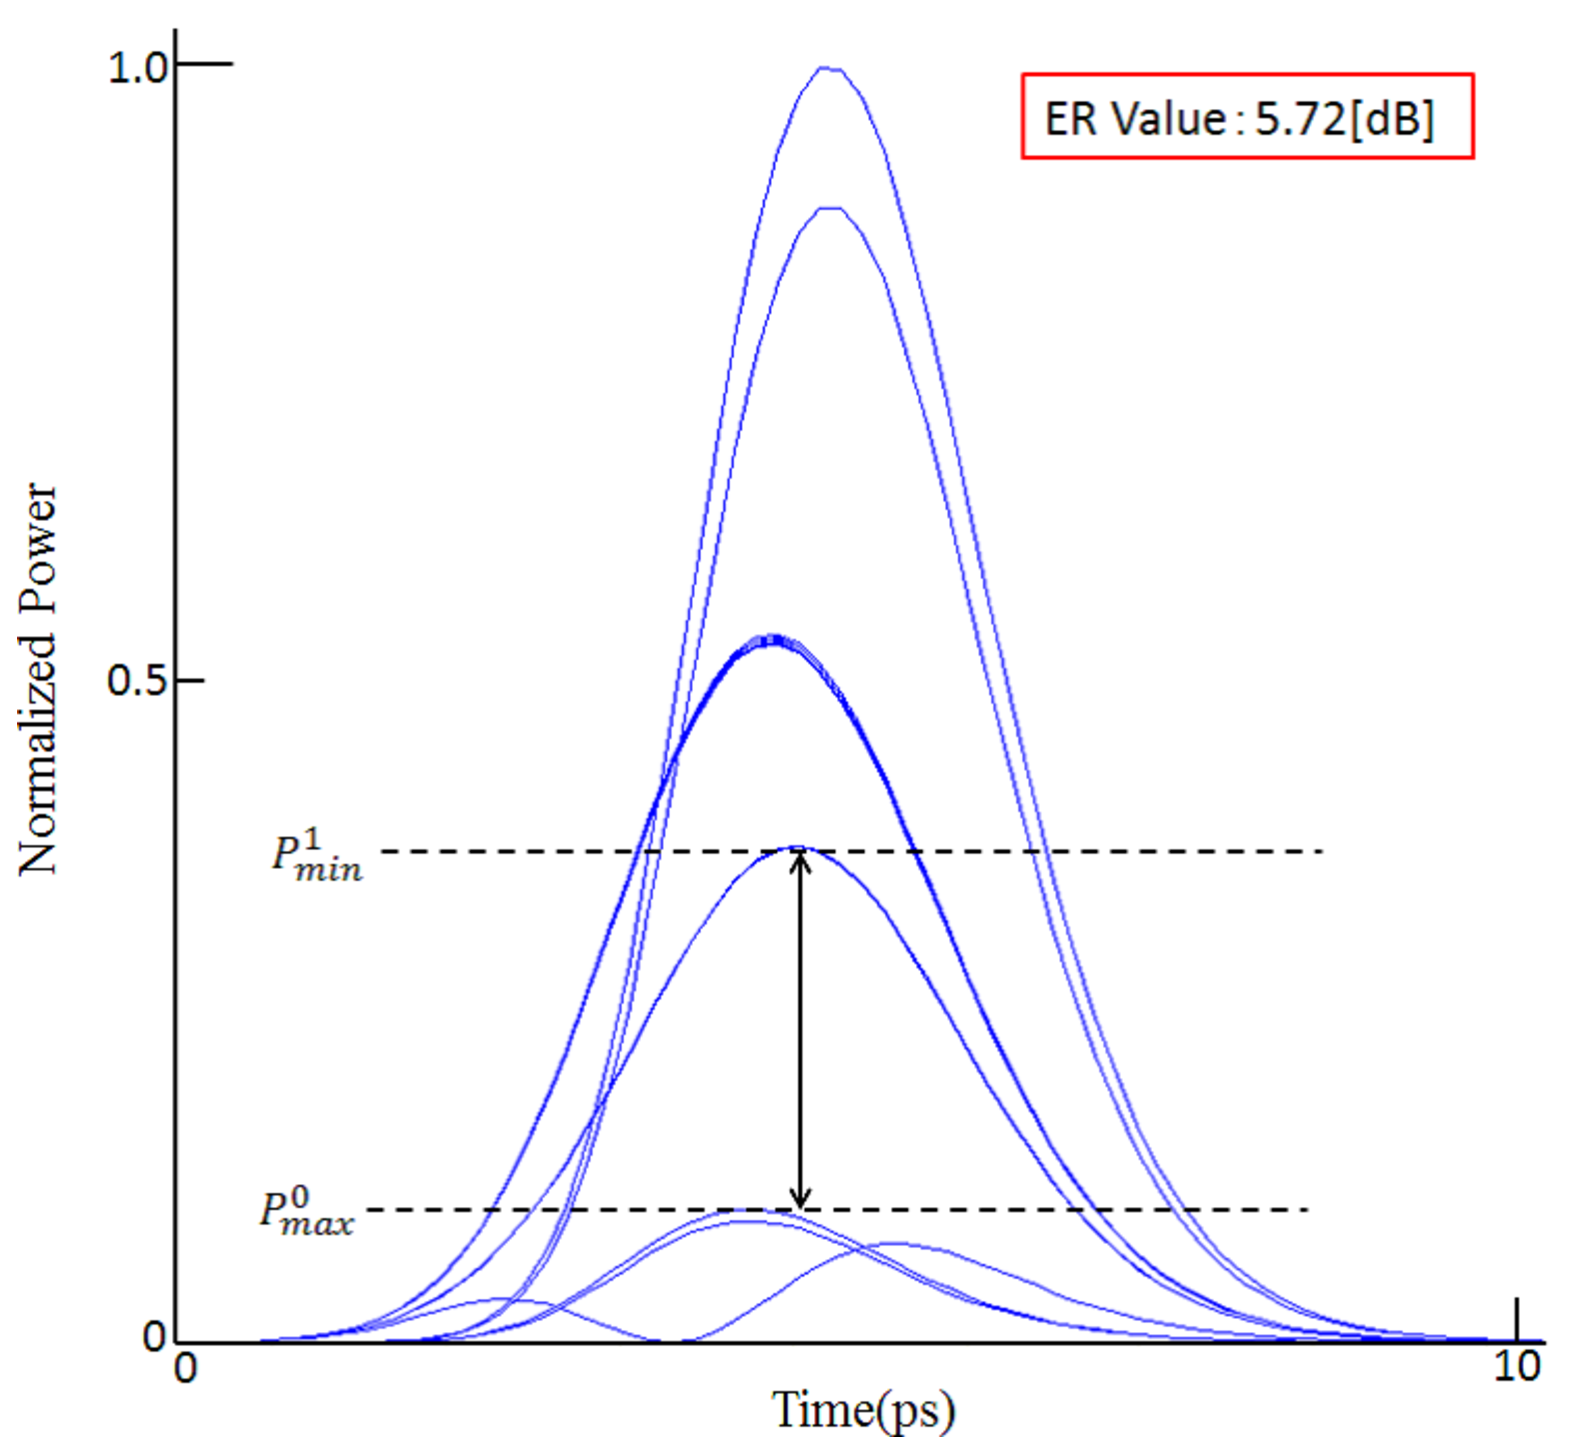
\includegraphics[width=60mm]{eyedia.eps}
  \caption{Eye diagram of decoded signal}
  \label{figure:eyedia}
\end{center}
\end{figure}

\section{Conclusion}
We have proposed an all optical encoder and decoder for error correcting code using horizontal and vertical parity checks and numerically analyzed the proposed system. We evaluate the performance of the proposed system by using eye diagram and extinction ratio. As a result, the proposed encoder and decoder obtain an encoded code and error corrected signal at 160Gbps, respectively, and it is shown that the proposed encoder and decoder obtain sufficient extinction ratio.

\begin{thebibliography}{9}
\bibitem{App} 
Y.Ben-Ezra, U.Mahlab, M.Haridim, and B.I.Lembrikov, ``Applications of All-Optical Signal Processing in Modern Optical Communications, "Proc. 9th International Conf. on Transparent Opt. Networks, no.Tu.B4.4, pp.328--331, Rome, The Italy, Jul. 2007.

\bibitem{Omar} 
Omar Qasaimeh, ``Theory of Four-Wave Mixing Wavelength Conversion in Quantum Dot Semiconductor Optical Amplifiers, " IEEE Photonics Technology Letters, vol.16, no.4, pp.993--995, Apr. 2004.

\bibitem{Ultrafast} 
Y.Ben-Ezra, B.I.Lembrikov, and M.Haridim, ``Ultrafast All-Optical  Processor Based on Quantum-Dot Semiconductor Optical Amplifiers, " IEEE Journal of Quantum Electronics, vol.45, no.1, pp.34--41, Jan. 2009.

\bibitem{80Gbps}
H.Dong, H.Sun, Q.Wang, N.K.Dutta, and J.Jaques, ``80 Gb/s All-optical logic AND operation using Mach-Zehnder interferometer with differential scheme, '' Optics Communications, vol.265, no.1, pp.79--83, Sep. 2006.

\bibitem{Rostami}
Ali Rostami, Hamed Baghban Asghari Nejad, Reza Maram Qartavol, and Hassan Rasooli Saghai, ``Tb/s Optical Logic Gates Based on Quantum-Dot Semiconductor Optical Amplifiers, " IEEE Journal of Quantum Electronics, vol.46, no.3, pp.354--360, Mar. 2010.

\bibitem{Gayen}
D.K.Gayen, A.Bhattachryya, T.Chattopadhyay, and J.N.Roy, ``Ultrafast All-Optical Half Adder Using Quantum-Dot Semiconductor Optical Amplifier-Based Mach-Zehnder Interferometer, " IEEE Journal of Lightwave Technology, vol.30, no.21, pp.3387--3393, Nov. 2012.

\end{thebibliography}
\end{document}



